\documentclass[11pt,a4paper]{article}

\usepackage[T1]{fontenc}
\usepackage{lmodern}
\usepackage[french]{babel}
\usepackage{amsmath,amssymb,amsthm}
\usepackage{geometry}
\usepackage{graphicx}
\usepackage{tikz}
\usepackage{pgfplots}
\pgfplotsset{compat=1.18}

\geometry{margin=2.5cm}

\newtheorem*{theoreme}{Théorème}

\title{Méthode des éléments finis en 2D}
\author{Mattis Duhaa}
\date{}

\begin{document}

\maketitle

\section{Introduction}

Ce document a pour but de décrire une méthode numérique de façon assez
précise pour qu'une IA puisse l'implémenter en Python.

Soit $\Omega$ un rectangle et $\beta \subset \Omega$ un obstacle (défini à la
section~\ref{sec:beta}). On pose $D = \Omega \setminus \beta$, dont le bord
est $\partial D = \partial\Omega \cup \partial\beta$. Pour $f \in L^2(D)$
donnée, on souhaite résoudre le problème
\[
(P)\quad
\begin{cases}
-\Delta u + u = f & \text{dans } D,\\[2pt]
u = 0 & \text{sur } \partial D .
\end{cases}
\]

\section{Formulation variationnelle}

On pose $V = H^1_0(D)$. Soit $v \in V$. On multiplie l'équation par $v$ et
on intègre sur $D$. La formule de Green donne
\[
\int_D -\Delta u \, v
= \int_D \nabla u \cdot \nabla v
- \underbrace{\int_{\partial D} \frac{\partial u}{\partial n}\, v \,\mathrm{d}s}_{=0 \text{ car } v = 0 \text{ sur } \partial D} ,
\]
d'où
\[
\int_D -\Delta u \, v + \int_D u\, v
= \int_D \nabla u \cdot \nabla v + \int_D u\, v .
\]
On définit
\begin{align*}
a(u, v) &= \int_D \nabla u \cdot \nabla v + \int_D u\, v,\\
\ell(v) &= \int_D f\, v.
\end{align*}

\paragraph{Problème continu.}
\[
(P_V)\quad \text{Trouver } u \in V \text{ tel que } a(u, v) = \ell(v)
\quad \forall v \in V .
\]

\paragraph{Problème discret.} Pour un espace de dimension finie
$V_h \subset V$ (défini à la section~\ref{sec:Vh}) :
\[
(P_h)\quad \text{Trouver } u_h \in V_h \text{ tel que } a(u_h, v_h) = \ell(v_h)
\quad \forall v_h \in V_h .
\]
La condition $u_h = 0$ sur $\partial D$ est contenue dans la définition de
$V_h$.

\begin{theoreme}[Lax--Milgram]
Soit $V$ un espace de Hilbert, $a$ une forme bilinéaire continue et
coercive sur $V$ et $\ell$ une forme linéaire continue sur $V$. Alors il
existe un unique $u \in V$ tel que $a(u,v) = \ell(v)$ pour tout $v \in V$.
\end{theoreme}

Ici $a$ est exactement le produit scalaire de $H^1(D)$. Par l'inégalité de
Cauchy--Schwarz,
\[
|a(u,v)| \le \|u\|_{H^1} \|v\|_{H^1},
\qquad
a(v,v) = \|v\|_{H^1}^2,
\qquad
|\ell(v)| \le \|f\|_{L^2} \|v\|_{H^1} .
\]
$a$ est donc continue et coercive (de constante $1$) et $\ell$ est continue.
Le théorème s'applique à $V$ et à $V_h$ : $(P_V)$ et $(P_h)$ ont chacun une
unique solution.

\paragraph{Estimation d'erreur (lemme de Céa).} En retranchant $(P_h)$ à
$(P_V)$ avec $v = v_h$, on obtient $a(u - u_h, v_h) = 0$ pour tout
$v_h \in V_h$. Comme $a$ est le produit scalaire de $H^1$, $u_h$ est la
projection orthogonale de $u$ sur $V_h$, donc
\[
\|u - u_h\|_{H^1} = \min_{v_h \in V_h} \|u - v_h\|_{H^1} .
\]
L'erreur ne dépend donc que de la capacité de $V_h$ à approcher $u$. Pour
des éléments de degré 2, on attend $\|u - u_h\|_{H^1} = O(h^2)$ et
$\|u - u_h\|_{L^2} = O(h^3)$.

\paragraph{Remarque.} Avec des triangles courbes, le domaine maillé $D_h$
n'est pas exactement $D$ : en toute rigueur $V_h \not\subset H^1_0(D)$.
L'erreur géométrique commise est d'un ordre supérieur et ne dégrade pas les
taux ci-dessus.


\section{Maillage en 2D}

L'idée est de réaliser un maillage autour d'un obstacle $\beta$ à bord
courbe, éventuellement non convexe, mais étoilé par rapport à un point $c$
(chaque demi-droite issue de $c$ coupe $\partial\beta$ une seule fois). Le
domaine $\Omega = [0, L_x] \times [0, L_y]$ est un rectangle, avec
$L_x = n_x h$ et $L_y = n_y h$, que l'on recouvre d'une grille cartésienne de
pas $h$. Le maillage couvre $\Omega \setminus \beta$, que l'on découpe en deux
zones :
\begin{itemize}
  \item une zone $\mathcal{Q}$, formée des cellules de la grille qui ne
        rencontrent pas $\beta$ et restent à une distance au moins $m_\beta$
        de $\beta$ ; ces cellules sont des quadrilatères (éléments $Q_2$) et
        recouvrent $\Omega$ jusqu'à son bord ;
  \item le reste $\mathcal{T} = (\Omega \setminus \beta) \setminus \mathcal{Q}$,
        une zone autour de $\beta$, remplie par une triangulation non
        structurée (éléments $P_2$), qui permet de suivre le bord courbe de
        $\beta$ et de raffiner le maillage à son voisinage.
\end{itemize}

Comme $\Omega$ est un rectangle aligné sur la grille, son bord est formé
d'arêtes de quadrilatères : aucun triangle n'est nécessaire le long de
$\partial\Omega$, et la condition $u = 0$ s'y impose directement sur les
nœuds de la grille.

\subsection{Définition de l'obstacle $\beta$}
\label{sec:beta}

On décrit $\beta$ en coordonnées polaires autour d'un centre
$c = (c_x, c_y)$. Pour $x \in \mathbb{R}^2$, on note
$\rho(x) = |x - c|$ et $\theta(x)$ l'angle polaire de $x - c$
(\texttt{numpy.arctan2}). On se donne un rayon $r(\theta) > 0$,
$2\pi$-périodique et régulier, et on pose
\[
\beta = \{ x : \rho(x) \le r(\theta(x)) \},
\qquad
\partial\beta = \{ \gamma(t),\ t \in [0, 2\pi) \},
\quad
\gamma(t) = c + r(t) \begin{pmatrix} \cos t \\ \sin t \end{pmatrix}.
\]
Deux formes sont utilisées :
\begin{itemize}
  \item \textbf{Disque} (validation) : $r(\theta) = R$.
  \item \textbf{Cacahuète} (non convexe) :
        $r(\theta) = r_0\,(1 + \varepsilon \cos 2\theta)$, avec
        $0 \le \varepsilon < 1$ pour que $r > 0$. Le bord est concave en
        $\theta = \pm\pi/2$ dès que $\varepsilon > 1/5$.
\end{itemize}
Les opérations géométriques dont le code a besoin sont alors :
\begin{itemize}
  \item \textbf{test d'appartenance} : $x \in \beta \iff \rho(x) \le r(\theta(x))$ ;
  \item \textbf{distance} $d(x, \beta)$ : distance minimale de $x$ à un
        échantillonnage fin de $\gamma$ (par exemple 2000 points), mise à
        zéro si $x \in \beta$ ;
  \item \textbf{fonction de niveau} $g_\beta(x) = \rho(x)^2 - r(\theta(x))^2$,
        négative dans $\beta$, nulle sur $\partial\beta$ et positive dans
        $D$. Elle est régulière dans $D$ car le centre $c$ est dans $\beta$.
\end{itemize}

\paragraph{Notations de taille.} Dans tout le document, $h$ désigne le pas
de la grille, $h_\beta$ le pas sur $\partial\beta$ et $\delta$ la largeur de
la zone de transition. Pour les études de convergence, on fait varier $h$ en
gardant $h_\beta / h$ et $\delta / h$ constants ; les estimations
$O(h^k)$ portent sur ce $h$.

\subsection{Construction du maillage}
\label{sec:construction}

Le maillage se construit ainsi :
\begin{enumerate}
  \item \textbf{Sélection des cellules.} On garde les cellules de la grille
        dont les quatre sommets et le centre sont hors de $\beta$ et à
        distance au moins $m_\beta$ de $\beta$. On retire ensuite, jusqu'à
        stabilisation, les cellules qui n'ont qu'une seule voisine (par une
        arête), ainsi que les deux cellules d'un sommet qui ne se touchent
        que par ce coin (sinon ce sommet serait partagé par quatre arêtes du
        bord de $\mathcal{Q}$).
  \item \textbf{Contour intérieur de $\mathcal{Q}$.} Les arêtes de la grille
        qui appartiennent à une seule cellule de $\mathcal{Q}$ forment deux contours fermés :
        $\partial\Omega$ et un contour polygonal autour de $\beta$, qui ne doit
        pas toucher $\partial\Omega$. Les nœuds de ce contour sont imposés :
        ce sont exactement les nœuds de la grille. Chacune de ses arêtes est
        donc commune à un quadrilatère et à un triangle, et le maillage est
        conforme : sur cette arête, les traces $Q_2$ et $P_2$ sont toutes deux
        quadratiques et partagent les trois mêmes nœuds (deux sommets et le
        milieu).
  \item \textbf{Bord de $\beta$.} On le discrétise avec un pas $h_\beta < h$,
        en répartissant les points selon l'abscisse curviligne, ce qui
        fonctionne pour un $\beta$ non convexe. En pratique, on calcule
        la longueur $s(t)$ de $\gamma$ sur un échantillonnage fin, on
        choisit $n_\beta = \lceil s(2\pi)/h_\beta \rceil$ points, et on
        garde pour chacun son paramètre $t_i$ (obtenu en inversant $s$).
  \item \textbf{Triangulation de $\mathcal{T}$.} On calcule une triangulation
        de Delaunay contrainte par ces deux contours, avec une taille de
        maille cible
        \[
        h_{\mathrm{loc}}(x) = h_\beta + (h - h_\beta)\,\min\!\left(1, \frac{d(x,\beta)}{\delta}\right),
        \]
        où $d(x,\beta)$ est la distance à $\beta$ et $\delta$ la largeur de
        la zone de transition. Les mailles sont ainsi fines près de $\beta$,
        où la solution varie le plus, et de taille $h$ au raccord avec la
        grille.
  \item \textbf{Éléments isoparamétriques.} Pour chaque arête posée sur
        $\partial\beta$, entre deux points de paramètres $t_a$ et $t_b$, le
        nœud milieu $P_2$ est placé sur $\partial\beta$ en
        $\gamma\big(\tfrac{t_a + t_b}{2}\big)$ (en tenant compte du passage
        de $2\pi$ à $0$ pour la dernière arête), et non au milieu du
        segment. Le triangle devient courbe, décrit par la
        transformation quadratique de l'élément de référence ; sans cela,
        l'erreur géométrique limiterait la convergence en norme $H^1$ à
        $O(h^{3/2})$ au lieu de $O(h^2)$.
\end{enumerate}

En pratique, on utilise le logiciel \texttt{gmsh} depuis Python. On lui donne
les deux contours (celui de $\beta$ et celui de la grille, dont les nœuds sont
fixés), puis il remplit la zone entre les deux avec des triangles, en suivant
la taille de maille $h_{\mathrm{loc}}(x)$ définie ci-dessus. La figure
ci-dessous est produite par \texttt{code/main.py} avec les paramètres par
défaut de la section~\ref{sec:parametres} ($\Omega = [0,7] \times [0,5]$,
$h = 0.5$, $h_\beta = 0.15$, $\delta = 0.8$, $m_\beta = 0.9$, obstacle en
forme de cacahuète) ; le maillage compte 108 quadrilatères et
214 triangles. Les arêtes posées sur $\partial\beta$ sont tracées courbes.

\begin{center}
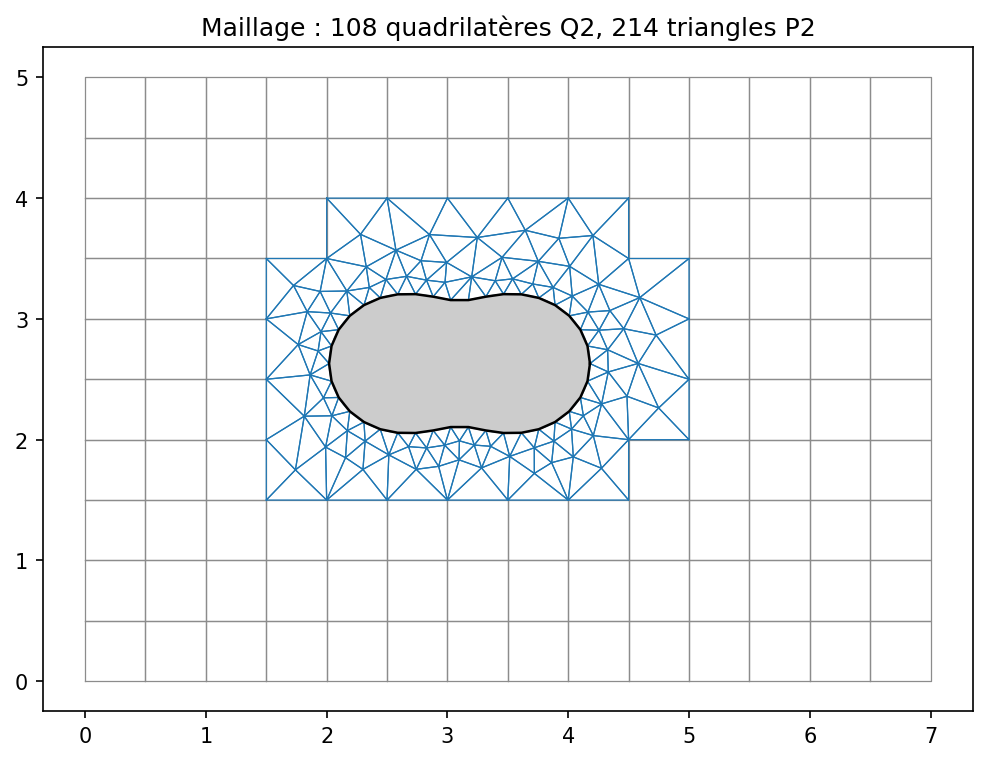
\includegraphics[width=0.85\textwidth]{code/resultats/maillage.png}
\end{center}

\subsection{Numérotation globale des nœuds}

La grille et \texttt{gmsh} numérotent leurs nœuds chacun de leur côté. On
construit une numérotation globale unique de la façon suivante :
\begin{enumerate}
  \item \textbf{Sommets de la grille.} Le sommet $(i h, j h)$,
        $0 \le i \le n_x$, $0 \le j \le n_y$, reçoit un numéro s'il est
        sommet d'au moins une cellule de $\mathcal{Q}$.
  \item \textbf{Sommets des triangles.} \texttt{gmsh} est appelé avec des
        éléments d'ordre 1 (triangles à 3 nœuds). Chaque point des deux
        contours est créé dans \texttt{gmsh} comme un point géométrique, et
        \texttt{gmsh} renvoie le nœud qui lui correspond : un nœud du
        contour intérieur de $\mathcal{Q}$ reprend le numéro du sommet de la
        grille, et un point de $\partial\beta$ reçoit un nouveau numéro en
        gardant son indice $k$ dans la discrétisation de $\gamma$. Les
        autres nœuds, intérieurs à $\mathcal{T}$, reçoivent un nouveau
        numéro.
  \item \textbf{Milieux d'arêtes.} On parcourt toutes les arêtes des
        triangles et des quadrilatères. Un dictionnaire, dont la clé est le
        couple trié $(\min(a,b), \max(a,b))$ des numéros des deux sommets,
        associe à chaque arête le numéro de son milieu. Le milieu n'est
        créé qu'à la première rencontre de l'arête : une arête commune à
        deux éléments (en particulier à un quadrilatère et à un triangle)
        a donc un seul milieu. Si l'arête est sur $\partial\beta$, le
        milieu est placé sur la courbe (étape 5 de la section~\ref{sec:construction}).
  \item \textbf{Centres des quadrilatères.} Chaque cellule de $\mathcal{Q}$
        reçoit un nœud supplémentaire en son centre.
  \item \textbf{Nœuds de bord.} Un nœud est sur $\partial\Omega$ si
        $x \in \{0, L_x\}$ ou $y \in \{0, L_y\}$ (à la tolérance près). Il
        est sur $\partial\beta$ s'il est un point de discrétisation de
        $\gamma$, ou le milieu d'une arête dont les deux sommets sont des
        points \emph{consécutifs} de cette discrétisation. Une arête qui
        relie deux points non voisins de $\partial\beta$ est une corde : elle
        traverse $D$ et son milieu reste un nœud intérieur.
\end{enumerate}

\subsection{Cas d'un obstacle polygonal}
\label{sec:polygone}

On considère maintenant un obstacle $\beta$ polygonal. Le reste de la
méthode (grille, zone $\mathcal{Q}$, triangulation de $\mathcal{T}$ par
\texttt{gmsh}, numérotation) est inchangé ; seules la description de
$\beta$, la discrétisation de son bord et le traitement des nœuds milieux
changent.

\paragraph{Définition.} On se donne $m$ sommets $P_1, \dots, P_m$, numérotés
dans le sens trigonométrique, et on pose $P_{m+1} = P_1$. Le polygone doit
être simple (ses côtés ne se coupent pas), mais il n'a pas besoin d'être
convexe ni étoilé. Le côté $j$ est le segment $[P_j, P_{j+1}]$, de longueur
$\ell_j = |P_{j+1} - P_j|$. On paramètre $\partial\beta$ par l'abscisse
curviligne : avec $s_1 = 0$, $s_{j+1} = s_j + \ell_j$ et
$L = s_{m+1}$ le périmètre,
\[
\gamma(s) = P_j + \frac{s - s_j}{\ell_j}\,(P_{j+1} - P_j)
\qquad \text{pour } s \in [s_j, s_{j+1}] .
\]
$\gamma$ est continue mais seulement affine par morceaux : elle n'est pas
dérivable aux sommets $P_j$.

\begin{center}
\begin{tikzpicture}[scale=1.6]
  % Obstacle carré
  \fill[gray!20] (0,0) rectangle (2,2);
  \draw[thick] (0,0) -- (2,0) -- (2,2) -- (0,2) -- cycle;
  \node at (1,1) {$\beta$};
  % Points de discrétisation (sommets inclus)
  \foreach \t in {0,0.5,1,1.5} {
    \fill (\t,0) circle (1pt);
    \fill (2,\t) circle (1pt);
    \fill (2-\t,2) circle (1pt);
    \fill (0,2-\t) circle (1pt);
  }
  \node[below left]  at (0,0) {$P_1$};
  \node[below right] at (2,0) {$P_2$};
  \node[below left]  at (2,2) {$P_3$};
  \node[above left]  at (0,2) {$P_4$};
  % Angle rentrant vu depuis D
  \draw[->] (2,1.65) arc (-90:180:0.35);
  \node at (2.75,2.45) {$\omega = \tfrac{3\pi}{2}$};
  \node at (3.2,1) {$D$};
\end{tikzpicture}
\end{center}

\paragraph{Opérations géométriques.} Elles remplacent celles de la
section~\ref{sec:beta} :
\begin{itemize}
  \item \textbf{test d'appartenance} : méthode du lancer de rayon. On compte
        le nombre de côtés coupés par la demi-droite horizontale issue de
        $x$ ; $x \in \beta$ si ce nombre est impair
        (\texttt{matplotlib.path.Path.contains\_points}) ;
  \item \textbf{distance} $d(x,\beta)$ : elle est maintenant exacte, sans
        échantillonnage. Pour chaque côté,
        \[
        d\big(x, [P_j, P_{j+1}]\big) = \big|x - P_j - \tau_j (P_{j+1} - P_j)\big|,
        \qquad
        \tau_j = \min\!\left(1, \max\!\left(0,
        \frac{(x - P_j)\cdot(P_{j+1} - P_j)}{\ell_j^2}\right)\right),
        \]
        puis $d(x,\beta) = \min_j d\big(x, [P_j, P_{j+1}]\big)$, mise à zéro si
        $x \in \beta$.
\end{itemize}

\paragraph{Discrétisation du bord.} On ne répartit plus les points
uniformément sur tout le périmètre : les sommets $P_j$ doivent être des
points de discrétisation, sinon le maillage \og couperait \fg{} les coins de
$\beta$. On découpe donc chaque côté séparément en
$n_j = \lceil \ell_j / h_\beta \rceil$ segments égaux :
\[
x_{j,i} = P_j + \frac{i}{n_j}\,(P_{j+1} - P_j),
\qquad 0 \le i < n_j .
\]
La liste de tous les $x_{j,i}$, dans l'ordre des côtés, donne les
$n_\beta = \sum_j n_j$ points de $\partial\beta$, que l'on transmet à
\texttt{gmsh} comme dans le cas courbe.

\paragraph{Éléments.} Chaque arête posée sur $\partial\beta$ relie deux
points consécutifs d'un même côté : elle est contenue dans $\partial\beta$.
Son nœud milieu est donc simplement le milieu du segment, et l'étape 5 de la
section~\ref{sec:construction} (placement sur $\gamma$) n'est plus
nécessaire. Tous les triangles sont à côtés droits : $\Phi_T$ est affine,
$|\det D\Phi_T| = 2|T|$ est constant, et la quadrature à 6 points calcule
$R^K$ et $M^K$ exactement. Le domaine maillé $D_h$ coïncide exactement avec
$D$ : il n'y a plus d'erreur géométrique et $V_h \subset H^1_0(D)$.

\paragraph{Exemple.} La figure ci-dessous est produite par
\texttt{code/main.py} avec les mêmes paramètres que pour la cacahuète
($\Omega = [0,7] \times [0,5]$, $h = 0.5$, $h_\beta = 0.15$, $\delta = 0.8$),
pour un obstacle en forme de L de sommets
\[
(2, 1.5),\ (5, 1.5),\ (5, 2.5),\ (3, 2.5),\ (3, 3.5),\ (2, 3.5).
\]
Ce polygone n'est pas convexe : il possède cinq coins saillants
($\alpha_j = \pi/2$, donc $\omega_j = 3\pi/2$ pour $D$) et un coin rentrant
en $(3, 2.5)$ ($\alpha_j = 3\pi/2$). Le maillage compte 68 quadrilatères et
435 triangles, sans raffinement aux coins. Les sommets du polygone sont bien
des nœuds du maillage, et toutes les arêtes posées sur $\partial\beta$ sont
droites.

\begin{center}
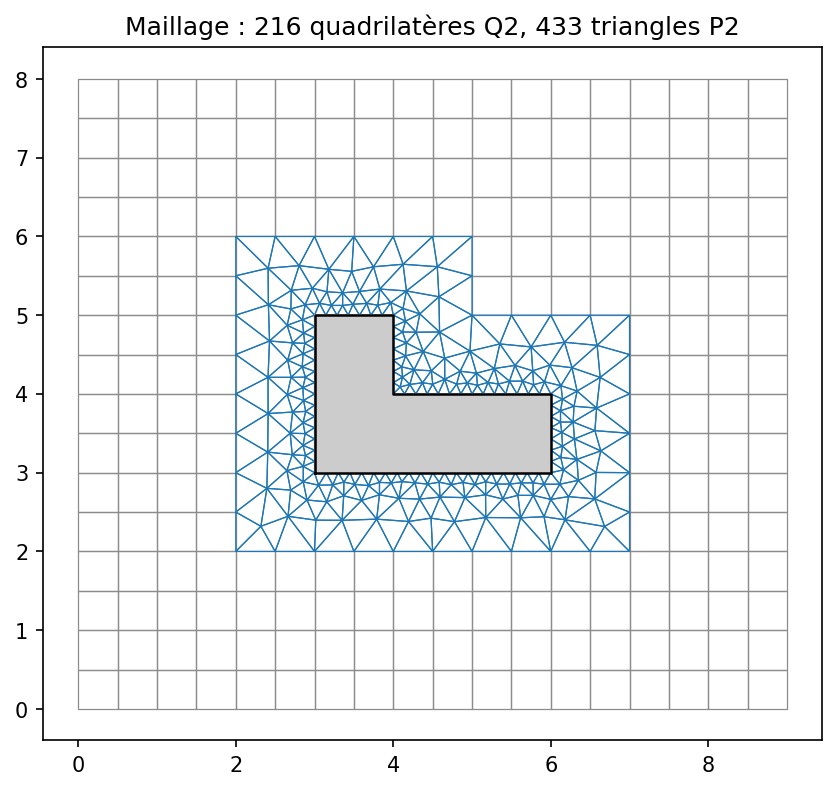
\includegraphics[width=0.85\textwidth]{code/resultats/maillage_polygone.png}
\end{center}

\paragraph{Singularités aux coins.} Un sommet $P_j$ où l'angle intérieur de
$\beta$ vaut $\alpha_j < \pi$ (coin saillant de $\beta$) est un coin
\emph{rentrant} pour $D$, d'angle $\omega_j = 2\pi - \alpha_j > \pi$. En
coordonnées polaires $(r, \theta)$ centrées en $P_j$, la solution se comporte
près de ce coin comme
\[
u(r, \theta) \sim C\, r^{\lambda_j} \sin(\lambda_j \theta),
\qquad \lambda_j = \frac{\pi}{\omega_j} < 1,
\]
dont le gradient est infini en $r = 0$. On a seulement
$u \in H^{1 + \lambda - \varepsilon}(D)$ pour tout $\varepsilon > 0$, avec
$\lambda = \min_j \lambda_j$. Sur un maillage à raffinement uniforme,
l'ordre $2$ des éléments finis ne sert plus à rien près du coin et on
observe
\[
\|u - u_h\|_{H^1} = O(h^{\lambda}),
\qquad
\|u - u_h\|_{L^2} = O(h^{2\lambda}).
\]
Pour un obstacle carré, $\omega = 3\pi/2$ et $\lambda = 2/3$ : on attend
$O(h^{2/3})$ en norme $H^1$ au lieu de $O(h^2)$. Seuls les sommets où
$\alpha_j > \pi$ (coins rentrants de $\beta$, donc saillants pour $D$) ne
posent pas de problème.

\paragraph{Raffinement aux coins.} Pour retrouver l'ordre optimal, on
raffine le maillage de façon graduée vers chaque sommet $P_j$ tel que
$\alpha_j < \pi$. Avec $r(x) = \min_j |x - P_j|$ (minimum pris sur ces
sommets), on remplace la taille cible par
\[
h_{\mathrm{loc}}^{\mathrm{coin}}(x)
= \max\!\left( h_{\min},\ \min\!\left( h_{\mathrm{loc}}(x),\
h_\beta \left(\frac{r(x)}{\delta}\right)^{1-\mu} \right) \right),
\]
où $h_{\mathrm{loc}}$ est la taille de la section~\ref{sec:construction}.
Pour des éléments de degré $k = 2$, le paramètre de gradation doit vérifier
$\mu < \lambda / k$, soit $\mu < 1/3$ pour un carré (on prend par exemple
$\mu = 1/4$). La taille minimale $h_{\min}$, de l'ordre de $h^{1/\mu}$,
évite une taille nulle au sommet. Le nombre de mailles reste de l'ordre de
$h^{-2}$ et on retrouve $O(h^2)$ en norme $H^1$ et $O(h^3)$ en norme $L^2$.
Il suffit de transmettre $h_{\mathrm{loc}}^{\mathrm{coin}}$ à \texttt{gmsh}
à la place de $h_{\mathrm{loc}}$ ; le reste du code est inchangé.

\paragraph{Validation.} Pour un obstacle rectangulaire
$\beta = [x_0, x_1] \times [y_0, y_1]$, on garde la solution manufacturée de
la section~\ref{sec:validation} en remplaçant $g$ par
\[
g(x,y) = X(x)\,Y(y),
\qquad X = (x - x_0)(x - x_1),
\qquad Y = (y - y_0)(y - y_1),
\]
qui s'annule sur $\partial\beta$ (ainsi que sur les prolongements des côtés,
ce qui ne gêne pas). On a $\nabla g = \big(X' Y,\ X Y'\big)$ avec
$X' = 2x - x_0 - x_1$, $Y' = 2y - y_0 - y_1$, et $\Delta g = 2(X + Y)$, d'où
\[
f = (1 + a^2 + b^2)\, S\, g - 2\, \nabla S \cdot \nabla g - S\, \Delta g .
\]
Cette solution est régulière : elle ne présente pas de singularité aux coins,
et l'on doit observer les ordres optimaux même sans raffinement aux coins.
Elle valide donc le code, mais pas le traitement des coins. Pour ce dernier,
on résout avec $f = 1$ et on compare à une solution de référence calculée sur
un maillage beaucoup plus fin : l'ordre observé doit passer de
$\lambda \approx 2/3$ (maillage uniforme) à $2$ (maillage gradué) en norme
$H^1$.

\section{Discrétisation}

\subsection{Espaces polynomiaux et espace $V_h$}
\label{sec:Vh}

On définit les espaces de polynômes $P_k$ (utilisés sur les triangles) et
$Q_k$ (utilisés sur les quadrilatères) :
\begin{align*}
P_k &= \left\{ p(x,y) = \sum_{m=0}^{k} \sum_{n=0}^{k-m} \alpha_{m,n}\, x^m y^n \right\},\\[4pt]
Q_k &= \left\{ p(x,y) = \sum_{m=0}^{k} \sum_{n=0}^{k} \alpha_{m,n}\, x^m y^n \right\}.
\end{align*}
On note $\mathcal{T}_h$ l'ensemble des triangles, $\mathcal{Q}_h$
l'ensemble des quadrilatères et $D_h$ le domaine qu'ils recouvrent. Avec les
transformations $\Phi_T$ et $\Phi_Q$ vers les éléments de référence
(section~\ref{sec:ref}), on pose
\[
V_h = \Big\{ v \in C^0(\overline{D_h}) \ :\
v|_T \circ \Phi_T \in P_2 \ \ \forall T \in \mathcal{T}_h,\ \
v|_Q \circ \Phi_Q \in Q_2 \ \ \forall Q \in \mathcal{Q}_h,\ \
v = 0 \text{ sur } \partial D_h \Big\}.
\]
Les fonctions de $V_h$ sont continues et polynomiales par morceaux, donc
dans $H^1(D_h)$. La continuité est assurée par le maillage : sur chaque
arête commune à deux éléments, les deux restrictions sont des polynômes de
degré 2 de l'abscisse le long de l'arête, qui coïncident en trois points
(les deux sommets et le milieu), donc partout. $V_h$ est engendré par les
fonctions de base nodales $\varphi_j$ (valant $1$ au nœud $j$ et $0$ aux
autres nœuds) associées aux nœuds qui ne sont pas sur $\partial D_h$.

\subsection{Passage à l'élément de référence}
\label{sec:ref}

Chaque élément $K$ du maillage est l'image d'un élément de référence
$\widehat{K}$ par une transformation $\Phi_K$ : le triangle $\widehat{T}$ de
sommets $(0,0)$, $(1,0)$, $(0,1)$ pour les triangles, le carré
$\widehat{Q} = [-1,1]^2$ pour les quadrilatères.

\begin{center}
\begin{tikzpicture}[scale=1.6]
  % Triangle de référence
  \draw (0,0) -- (1,0) -- (0,1) -- cycle;
  \node[below left]  at (0,0) {$(0,0)$};
  \node[below right] at (1,0) {$(1,0)$};
  \node[above]       at (0,1) {$(0,1)$};
  \node at (0.5,-0.45) {$\widehat{T}$};

  % Flèche
  \draw[->, thick] (1.4,0.5) -- (2.4,0.5) node[midway, above] {$\Phi_T$};

  % Triangle T
  \begin{scope}[shift={(2.8,0)}]
    \draw (0,0) -- (1.3,0.1) -- (0.6,0.9) -- cycle;
    \node[below left]  at (0,0)       {$(x_1,y_1)$};
    \node[below right] at (1.3,0.1)   {$(x_2,y_2)$};
    \node[above]       at (0.6,0.9)   {$(x_3,y_3)$};
    \node at (0.65,-0.45) {$T$};
  \end{scope}
\end{tikzpicture}
\end{center}

\begin{center}
\begin{tikzpicture}[scale=1.3]
  % Carré de référence
  \draw (-1,-1) -- (1,-1) -- (1,1) -- (-1,1) -- cycle;
  \node[below left]  at (-1,-1) {$(-1,-1)$};
  \node[below right] at (1,-1)  {$(1,-1)$};
  \node[above right] at (1,1)   {$(1,1)$};
  \node[above left]  at (-1,1)  {$(-1,1)$};
  \node at (0,0) {$\widehat{Q}$};

  % Flèche
  \draw[->, thick] (1.6,0) -- (2.8,0) node[midway, above] {$\Phi_Q$};

  % Quadrilatère Q
  \begin{scope}[shift={(3.4,-1)}]
    \draw (0,0) -- (2.2,0.2) -- (2.5,1.9) -- (0.3,1.6) -- cycle;
    \node[below left]  at (0,0)       {$(x_1,y_1)$};
    \node[below right] at (2.2,0.2)   {$(x_2,y_2)$};
    \node[above right] at (2.5,1.9)   {$(x_3,y_3)$};
    \node[above left]  at (0.3,1.6)   {$(x_4,y_4)$};
    \node at (1.25,0.95) {$Q$};
  \end{scope}
\end{tikzpicture}
\end{center}

On décrit la géométrie avec les mêmes fonctions de base que la solution
(éléments \emph{isoparamétriques}). Si $K$ a $n_K$ nœuds $x_k$ ($n_K = 6$
pour un triangle, $n_K = 9$ pour un quadrilatère) et si $\widehat{\psi}_k$
sont les fonctions $P_2$ ou $Q_2$ de la section~\ref{sec:bases} :
\[
\Phi_K(\hat{x}) = \sum_{k=1}^{n_K} x_k\, \widehat{\psi}_k(\hat{x}),
\qquad
D\Phi_K(\hat{x}) = \sum_{k=1}^{n_K} x_k\, \nabla\widehat{\psi}_k(\hat{x})^{\top}
\quad (\text{matrice } 2 \times 2).
\]
Pour toute fonction $\varphi$ définie sur $K$, on note
$\widehat{\varphi} = \varphi \circ \Phi_K$. La dérivation des fonctions
composées et le changement de variables donnent
\[
\nabla \varphi \circ \Phi_K = D\Phi_K^{-\top}\, \nabla \widehat{\varphi},
\qquad
\int_K g \,\mathrm{d}x = \int_{\widehat{K}} g \circ \Phi_K\,
\left|\det D\Phi_K\right| \,\mathrm{d}\hat{x} .
\]
En particulier, si le nœud global $i$ est le nœud local $k$ de $K$, alors
$\varphi_i \circ \Phi_K = \widehat{\psi}_k$ : toutes les intégrales se calculent
avec les fonctions de référence.

\paragraph{Cas particuliers.}
\begin{itemize}
  \item \textbf{Triangle à côtés droits} (milieux au milieu des arêtes) : $\Phi_T$ est
        affine,
        \[
        \Phi_T(\hat{x}) = x_1 + \big[\, x_2 - x_1 \ \big|\ x_3 - x_1 \,\big]\, \hat{x},
        \qquad \left|\det D\Phi_T\right| = 2\,|T| .
        \]
  \item \textbf{Carré de la grille} de côté $h$ et de centre $x_c$ :
        \[
        \Phi_Q(\hat{x}) = x_c + \tfrac{h}{2}\, \hat{x},
        \qquad D\Phi_Q = \tfrac{h}{2} I,
        \qquad \left|\det D\Phi_Q\right| = \tfrac{h^2}{4} .
        \]
  \item \textbf{Triangle courbe} (une arête sur $\partial\beta$, milieu placé
        sur la courbe) : $\Phi_T$ est quadratique et $D\Phi_T$ dépend du point.
        C'est ce qui permet à l'élément de suivre le bord de $\beta$.
\end{itemize}

\section{Système linéaire et structure des matrices}

\subsection{Du problème discret au système linéaire}

On note $N$ le nombre total de nœuds du maillage (sommets, milieux
d'arêtes et centres des quadrilatères), y compris les nœuds de bord, et
$(\varphi_j)_{1 \le j \le N}$ les fonctions nodales associées, avec
$\varphi_j = 1$ au nœud $j$ et $0$ aux autres. Seules celles des nœuds
intérieurs forment une base de $V_h$ ; on travaille d'abord avec toutes,
et les nœuds de bord sont éliminés à la section~\ref{sec:dirichlet}.
On cherche
\[
u_h = \sum_{j=1}^{N} U_j\, \varphi_j ,
\qquad U = (U_1,\dots,U_N)^\top \in \mathbb{R}^N .
\]
En prenant $v_h = \varphi_i$ dans $(P_h)$ pour $i = 1,\dots,N$, on obtient
le système linéaire
\[
\boxed{\ A\,U = F, \qquad A = R + M\ }
\]
avec
\[
R_{ij} = \int_D \nabla\varphi_j \cdot \nabla\varphi_i ,
\qquad
M_{ij} = \int_D \varphi_j\, \varphi_i ,
\qquad
F_i = \int_D f\, \varphi_i .
\]
$R$ est la matrice de rigidité, $M$ la matrice de masse et $F$ le second
membre. On a $A_{ij} = a(\varphi_j, \varphi_i)$ : $A$ est donc symétrique
définie positive.

\subsection{Fonctions de base $P_2$ et $Q_2$ sur les éléments de référence}
\label{sec:bases}

Les fonctions de degré 2 $\widehat{\psi}_k$ servent à la fois à approcher
$u$ et à décrire la géométrie des éléments (section~\ref{sec:ref}).

\paragraph{Triangle $P_2$ (6 nœuds).} Sur $\widehat{T}$, avec
$\lambda_1 = 1 - \hat{x} - \hat{y}$, $\lambda_2 = \hat{x}$,
$\lambda_3 = \hat{y}$, les nœuds sont numérotés : sommets $1{:}(0,0)$,
$2{:}(1,0)$, $3{:}(0,1)$, puis milieux $4{:}(\tfrac12,0)$,
$5{:}(\tfrac12,\tfrac12)$, $6{:}(0,\tfrac12)$.
\[
\begin{aligned}
\widehat{\psi}_1 &= \lambda_1(2\lambda_1 - 1), &
\nabla\widehat{\psi}_1 &= (4\lambda_1 - 1)\begin{pmatrix} -1 \\ -1 \end{pmatrix}, \\
\widehat{\psi}_2 &= \hat{x}(2\hat{x} - 1), &
\nabla\widehat{\psi}_2 &= \begin{pmatrix} 4\hat{x} - 1 \\ 0 \end{pmatrix}, \\
\widehat{\psi}_3 &= \hat{y}(2\hat{y} - 1), &
\nabla\widehat{\psi}_3 &= \begin{pmatrix} 0 \\ 4\hat{y} - 1 \end{pmatrix}, \\
\widehat{\psi}_4 &= 4\lambda_1\hat{x}, &
\nabla\widehat{\psi}_4 &= 4\begin{pmatrix} 1 - 2\hat{x} - \hat{y} \\ -\hat{x} \end{pmatrix}, \\
\widehat{\psi}_5 &= 4\hat{x}\hat{y}, &
\nabla\widehat{\psi}_5 &= 4\begin{pmatrix} \hat{y} \\ \hat{x} \end{pmatrix}, \\
\widehat{\psi}_6 &= 4\lambda_1\hat{y}, &
\nabla\widehat{\psi}_6 &= 4\begin{pmatrix} -\hat{y} \\ 1 - \hat{x} - 2\hat{y} \end{pmatrix}.
\end{aligned}
\]

\paragraph{Quadrilatère $Q_2$ (9 nœuds).} Sur $\widehat{Q} = [-1,1]^2$, on
utilise les polynômes de Lagrange 1D de degré 2 aux points $-1, 0, 1$ :
\[
\ell_{-1}(s) = \tfrac12 s(s-1), \qquad
\ell_{0}(s) = 1 - s^2, \qquad
\ell_{1}(s) = \tfrac12 s(s+1),
\]
\[
\ell_{-1}'(s) = s - \tfrac12, \qquad
\ell_{0}'(s) = -2s, \qquad
\ell_{1}'(s) = s + \tfrac12 .
\]
Les nœuds sont numérotés : sommets $1{:}(-1,-1)$, $2{:}(1,-1)$,
$3{:}(1,1)$, $4{:}(-1,1)$, milieux $5{:}(0,-1)$, $6{:}(1,0)$, $7{:}(0,1)$,
$8{:}(-1,0)$, et centre $9{:}(0,0)$. Si le nœud $k$ a pour coordonnées
$(a_k, b_k)$, alors
\[
\widehat{\psi}_k(\hat{x},\hat{y}) = \ell_{a_k}(\hat{x})\,\ell_{b_k}(\hat{y}),
\qquad
\nabla\widehat{\psi}_k =
\begin{pmatrix}
\ell_{a_k}'(\hat{x})\,\ell_{b_k}(\hat{y}) \\
\ell_{a_k}(\hat{x})\,\ell_{b_k}'(\hat{y})
\end{pmatrix}.
\]

\subsection{Quadrature}

Les intégrales sur l'élément de référence sont approchées par
\[
\int_{\widehat{K}} g(\hat{x}) \,\mathrm{d}\hat{x}
\approx \sum_{q=1}^{n_q} w_q\, g(\hat{x}_q).
\]
\begin{itemize}
  \item \textbf{Triangle} : règle de Gauss à 6 points, exacte pour les
        polynômes de degré 4. Avec $a = 0.445948490915965$ et
        $b = 0.091576213509771$, les points sont
        \[
        (a,a),\ (1-2a,a),\ (a,1-2a) \quad \text{de poids } w_a = 0.111690794839005,
        \]
        \[
        (b,b),\ (1-2b,b),\ (b,1-2b) \quad \text{de poids } w_b = 0.054975871827661.
        \]
        La somme des poids vaut $\tfrac12$, l'aire de $\widehat{T}$.
  \item \textbf{Quadrilatère} : Gauss--Legendre $3 \times 3$. Les points
        sont les $(s_m, s_n)$ et les poids les produits $w_m w_n$, avec
        \[
        s \in \{-\sqrt{3/5},\ 0,\ \sqrt{3/5}\},
        \qquad
        w \in \{\tfrac59,\ \tfrac89,\ \tfrac59\}.
        \]
\end{itemize}
Les valeurs $\widehat{\psi}_k(\hat{x}_q)$ et $\nabla\widehat{\psi}_k(\hat{x}_q)$
ne dépendent pas de l'élément : on les calcule une seule fois.

\subsection{Matrices élémentaires}

Pour un élément $K$ à $n_K$ nœuds ($n_K = 6$ pour un triangle,
$n_K = 9$ pour un quadrilatère), de transformation $\Phi_K$, on note en
chaque point de quadrature $\hat{x}_q$ :
\begin{itemize}
  \item $J_q = D\Phi_K(\hat{x}_q)$ et $d_q = |\det J_q|$ ;
  \item $\Psi_q = \big(\widehat{\psi}_1(\hat{x}_q), \dots, \widehat{\psi}_{n_K}(\hat{x}_q)\big)^{\top} \in \mathbb{R}^{n_K}$ ;
  \item $G_q = \big[\nabla\widehat{\psi}_1(\hat{x}_q) \ \cdots\ \nabla\widehat{\psi}_{n_K}(\hat{x}_q)\big] \in \mathbb{R}^{2 \times n_K}$ ;
  \item $B_q = J_q^{-\top} G_q \in \mathbb{R}^{2 \times n_K}$, qui contient
        les gradients des fonctions de base sur l'élément réel.
\end{itemize}
Les matrices et le vecteur élémentaires s'écrivent alors
\[
R^K = \sum_{q} w_q\, d_q\, B_q^{\top} B_q ,
\qquad
M^K = \sum_{q} w_q\, d_q\, \Psi_q \Psi_q^{\top} ,
\qquad
F^K = \sum_{q} w_q\, d_q\, f\big(\Phi_K(\hat{x}_q)\big)\, \Psi_q ,
\]
avec $R^K, M^K \in \mathbb{R}^{n_K \times n_K}$ symétriques et
$F^K \in \mathbb{R}^{n_K}$. On pose $A^K = R^K + M^K$.

\paragraph{Cas des carrés de la grille.} Pour une cellule de côté $h$,
$J_q = \tfrac{h}{2} I$ et $d_q = \tfrac{h^2}{4}$ en tout point. On obtient
\[
R^K = \widehat{R}, \qquad M^K = \frac{h^2}{4}\, \widehat{M},
\]
où $\widehat{R}$ et $\widehat{M}$ sont calculées sur $\widehat{Q}$ avec
$d_q = 1$ et $B_q = G_q$. Elles sont identiques pour tous les
quadrilatères : il suffit de les calculer une seule fois.

\subsection{Assemblage}

Chaque élément $K$ possède une table de connectivité
$\mathrm{conn}_K(k)$ qui donne le numéro global du nœud local $k$. Un nœud
partagé par plusieurs éléments (sommet ou milieu d'arête) a un seul numéro
global. L'assemblage consiste à ajouter chaque contribution élémentaire à
la bonne place :
\begin{enumerate}
  \item Initialiser $A = 0 \in \mathbb{R}^{N \times N}$ et
        $F = 0 \in \mathbb{R}^{N}$.
  \item Pour chaque élément $K$ (triangles puis quadrilatères) :
        \begin{enumerate}
          \item calculer $A^K$ et $F^K$ ;
          \item pour $k, l = 1, \dots, n_K$ :
                $A_{\mathrm{conn}_K(k),\,\mathrm{conn}_K(l)} \mathrel{+}= A^K_{kl}$ ;
          \item pour $k = 1, \dots, n_K$ :
                $F_{\mathrm{conn}_K(k)} \mathrel{+}= F^K_k$.
        \end{enumerate}
\end{enumerate}

\paragraph{Structure de $A$.} $A_{ij} \neq 0$ seulement si les nœuds $i$ et
$j$ appartiennent à un même élément. $A$ est donc \emph{creuse} : chaque
ligne contient au plus quelques dizaines de termes non nuls (25 pour un
sommet commun à quatre quadrilatères $Q_2$), quel que soit $N$. En Python,
on stocke les triplets $(i, j, A^K_{kl})$ dans trois listes, puis on
construit la matrice au format \texttt{scipy.sparse.coo\_matrix}, qui
additionne automatiquement les doublons, avant de la convertir au format
CSR pour la résolution.

\subsection{Conditions aux limites et système final}
\label{sec:dirichlet}

On sépare les nœuds en deux ensembles :
\begin{itemize}
  \item $\mathcal{I}$ : les nœuds intérieurs ;
  \item $\mathcal{B}$ : les nœuds situés sur $\partial\Omega$ ou sur
        $\partial\beta$ (y compris les milieux $P_2$ placés sur la courbe
        $\partial\beta$).
\end{itemize}
En renumérotant les inconnues dans cet ordre, le système s'écrit par blocs
\[
\begin{pmatrix}
A_{\mathcal{I}\mathcal{I}} & A_{\mathcal{I}\mathcal{B}} \\
A_{\mathcal{B}\mathcal{I}} & A_{\mathcal{B}\mathcal{B}}
\end{pmatrix}
\begin{pmatrix} U_{\mathcal{I}} \\ U_{\mathcal{B}} \end{pmatrix}
=
\begin{pmatrix} F_{\mathcal{I}} \\ F_{\mathcal{B}} \end{pmatrix}.
\]
La condition $u = 0$ sur $\partial D$ impose $U_{\mathcal{B}} = 0$. Les
lignes associées à $\mathcal{B}$ ne sont plus des équations à résoudre, et
il reste
\[
\boxed{\ A_{\mathcal{I}\mathcal{I}}\, U_{\mathcal{I}} = F_{\mathcal{I}}\ }
\]
$A_{\mathcal{I}\mathcal{I}}$ est symétrique définie positive, donc le système
admet une unique solution. On le résout avec
\texttt{scipy.sparse.linalg.spsolve} (ou un gradient conjugué), puis on
reconstruit $U$ en complétant par $U_{\mathcal{B}} = 0$.

\subsection{Récapitulatif des tableaux}

\begin{center}
\begin{tabular}{lll}
\hline
Nom & Taille & Contenu \\
\hline
\texttt{coords} & $N \times 2$ & coordonnées $(x,y)$ de chaque nœud \\
\texttt{tri}    & $n_T \times 6$ & numéros globaux des nœuds de chaque triangle \\
\texttt{quad}   & $n_Q \times 9$ & numéros globaux des nœuds de chaque quadrilatère \\
\texttt{bnd}    & $|\mathcal{B}|$ & indices des nœuds de $\partial\Omega \cup \partial\beta$ \\
$A^K$, $F^K$    & $n_K \times n_K$, $n_K$ & matrice et vecteur élémentaires \\
$A$             & $N \times N$ (creuse) & $R + M$ assemblée \\
$F$             & $N$ & second membre assemblé \\
$U$             & $N$ & valeurs de $u_h$ aux nœuds \\
\hline
\end{tabular}
\end{center}

L'ordre des nœuds locaux dans \texttt{tri} et \texttt{quad} doit être le
même que celui des éléments de référence ci-dessus.

\section{Validation}
\label{sec:validation}

\subsection{Solution manufacturée}

Pour vérifier le code, on choisit une solution exacte $u_{\mathrm{ex}}$ qui
s'annule sur $\partial\Omega$ et sur $\partial\beta$, et on en déduit $f$.
On prend $\Omega = [0, L_x] \times [0, L_y]$ et pour $\beta$ le disque de
centre $c$ et de rayon $R$. Avec $a = \pi / L_x$ et $b = \pi / L_y$ :
\[
S(x,y) = \sin(a x)\sin(b y),
\qquad
g(x,y) = (x - c_x)^2 + (y - c_y)^2 - R^2,
\qquad
u_{\mathrm{ex}} = S\, g .
\]
$S$ s'annule sur $\partial\Omega$ et $g$ sur $\partial\beta$. On a
\[
\nabla u_{\mathrm{ex}} = g\, \nabla S + S\, \nabla g,
\qquad
\nabla S = \begin{pmatrix} a \cos(a x)\sin(b y) \\ b \sin(a x)\cos(b y) \end{pmatrix},
\qquad
\nabla g = 2 \begin{pmatrix} x - c_x \\ y - c_y \end{pmatrix},
\]
et, avec $\Delta S = -(a^2 + b^2) S$ et $\Delta g = 4$,
\[
f = -\Delta u_{\mathrm{ex}} + u_{\mathrm{ex}}
= (1 + a^2 + b^2)\, S\, g
- 4\big[ a (x - c_x) \cos(a x)\sin(b y) + b (y - c_y) \sin(a x)\cos(b y) \big]
- 4 S .
\]

\subsection{Calcul des erreurs}

Les erreurs sont calculées élément par élément avec la même quadrature que
pour l'assemblage. Avec les notations de la section sur les matrices
élémentaires, et $U^K = (U_{\mathrm{conn}_K(k)})_{k}$ les valeurs de $u_h$
aux nœuds de l'élément $K$ :
\[
\|u_{\mathrm{ex}} - u_h\|_{L^2}^2
\approx \sum_{K} \sum_{q} w_q\, d_q
\Big( u_{\mathrm{ex}}(x_q) - \Psi_q^{\top} U^K \Big)^2 ,
\]
\[
|u_{\mathrm{ex}} - u_h|_{H^1}^2
\approx \sum_{K} \sum_{q} w_q\, d_q
\Big| \nabla u_{\mathrm{ex}}(x_q) - B_q\, U^K \Big|^2 ,
\]
où $x_q = \Phi_K(\hat{x}_q)$. On a
$\|u_{\mathrm{ex}} - u_h\|_{H^1}^2 = \|u_{\mathrm{ex}} - u_h\|_{L^2}^2
+ |u_{\mathrm{ex}} - u_h|_{H^1}^2$.

\subsection{Étude de convergence}

On résout le problème pour $h \in \{0.5,\ 0.25,\ 0.125,\ 0.0625\}$, en
gardant $h_\beta = 0.3\,h$, $\delta = 1.6\,h$ et $m_\beta = 0.9\,h$. Pour deux
pas successifs $h$ et $h/2$, l'ordre observé, pour une erreur $E(h)$, est
\[
p = \frac{\log\big(E(h) / E(h/2)\big)}{\log 2} .
\]
On doit observer $p \approx 3$ pour l'erreur $L^2$ et $p \approx 2$ pour
l'erreur $H^1$. Un ordre $H^1$ proche de $1.5$ indique en général que les
milieux des arêtes de $\partial\beta$ ne sont pas placés sur la courbe. Un
ordre proche de $1$ ou une erreur qui ne diminue pas indique une erreur
dans les fonctions de base, la numérotation locale ou l'assemblage.

\subsection{Cas d'application}

Une fois le code validé, on le lance sur l'obstacle en forme de cacahuète
avec $f = 1$. Il n'y a pas de solution exacte : on vérifie seulement que
$u_h$ est positive, nulle sur $\partial D$ et régulière.

\section{Paramètres et sorties attendues}

\subsection{Paramètres par défaut}
\label{sec:parametres}

\begin{center}
\begin{tabular}{lll}
\hline
Paramètre & Valeur & Rôle \\
\hline
$L_x$, $L_y$     & $7$, $5$     & dimensions de $\Omega$ ($L_x/h$, $L_y/h$ entiers) \\
$h$              & $0.5$        & pas de la grille \\
$h_\beta$        & $0.15$       & pas sur $\partial\beta$ \\
$\delta$         & $0.8$        & largeur de la zone de transition \\
$m_\beta$        & $0.9$       & distance minimale entre $\mathcal{Q}$ et $\beta$ \\
disque           & $c = (3.5, 2.5)$, $R = 1$ & obstacle de validation \\
cacahuète        & $c = (3.1, 2.63)$, $r_0 = 0.8$, & obstacle d'application \\
                 & $\varepsilon = 0.35$ & \\
\hline
\end{tabular}
\end{center}

\subsection{Organisation du code}

\begin{center}
\begin{tabular}{ll}
\hline
Module & Contenu \\
\hline
\texttt{geometry.py}  & $r(\theta)$, $\gamma(t)$, test $x \in \beta$, $d(x,\beta)$, $g_\beta$ \\
\texttt{mesh.py}      & sélection de $\mathcal{Q}$, appel à \texttt{gmsh}, numérotation, nœuds P2/Q2 \\
\texttt{reference.py} & $\widehat{\psi}_k$, $\nabla\widehat{\psi}_k$, points et poids de quadrature \\
\texttt{assembly.py}  & $\Phi_K$, $D\Phi_K$, $R^K$, $M^K$, $F^K$, assemblage creux \\
\texttt{solver.py}    & élimination des nœuds de $\mathcal{B}$, résolution \\
\texttt{main.py}      & cas de validation, étude de convergence, figures \\
\hline
\end{tabular}
\end{center}

Dépendances : \texttt{numpy}, \texttt{scipy}, \texttt{gmsh}, \texttt{matplotlib}.

\subsection{Sorties}

\begin{itemize}
  \item \texttt{maillage.png} : les quadrilatères, les triangles et $\beta$
        (\texttt{maillage\_polygone.png} pour l'obstacle polygonal).
  \item \texttt{solution.png} : $u_h$ en couleurs. Pour l'affichage, chaque
        triangle $P_2$ est découpé en 4 sous-triangles et chaque carré $Q_2$
        en 8 à l'aide des nœuds milieux, puis on trace le résultat avec
        \texttt{matplotlib.pyplot.tripcolor}. Une triangulation de Delaunay
        de tous les nœuds ne convient pas : elle traverserait $\beta$.
  \item \texttt{convergence.png} : erreurs $L^2$ et $H^1$ en fonction de
        $h$ en échelle log--log, avec des droites de pente 3 et 2.
  \item Dans le terminal : le nombre de nœuds, de triangles et de
        quadrilatères, puis un tableau $h$, erreur $L^2$, ordre, erreur
        $H^1$, ordre.
\end{itemize}

\end{document}
